% ============================================================
% Question Bank: ch02-06 Simple Interest (Modified)
% Topic Title: Simple Interest (Florida / Texas Emphasis)
% CCSS: 7.RP.A.3
% Questions: 27 (15 MC + 6 SA + 6 Graphical)
% ============================================================

% --- Multiple Choice Questions (15) ---

\begin{practiceQuestion}{m-2-6-q01}{mc}
\begin{questionText}
You deposit $\$1{,}200$ in a savings account that earns $3\%$ simple interest per year. How much interest do you earn after $4$ years?
\end{questionText}
\choiceA{$\$36$}
\choiceB{$\$48$}
\choiceC{$\$144$}
\choiceD{$\$1{,}344$}
\correctAnswer{C}
\explanation{$I = 1{,}200 \times 0.03 \times 4 = \$144$.}
\end{practiceQuestion}

\begin{practiceQuestion}{m-2-6-q02}{mc}
\begin{questionText}
A student borrows $\$750$ for school supplies at $5\%$ simple interest for $2$ years. What is the total amount she must repay?
\end{questionText}
\choiceA{$\$75$}
\choiceB{$\$787.50$}
\choiceC{$\$825$}
\choiceD{$\$1{,}500$}
\correctAnswer{C}
\explanation{$I = 750 \times 0.05 \times 2 = \$75$. Total: $750 + 75 = \$825$.}
\end{practiceQuestion}

\begin{practiceQuestion}{m-2-6-q03}{mc}
\begin{questionText}
Which is the best reason to compare interest rates at different banks before opening a savings account?
\end{questionText}
\choiceA{Higher rates always mean higher fees}
\choiceB{A higher interest rate earns you more money on your deposit}
\choiceC{All banks pay the same rate}
\choiceD{Interest rates do not affect your savings}
\correctAnswer{B}
\explanation{A higher interest rate means your money grows faster. Comparing rates helps you maximize earnings on your savings.}
\end{practiceQuestion}

\begin{practiceQuestion}{m-2-6-q04}{mc}
\begin{questionText}
Bank A offers $2\%$ simple interest. Bank B offers $3.5\%$ simple interest. You deposit $\$2{,}000$ for $3$ years. How much more does Bank B earn you?
\end{questionText}
\choiceA{$\$30$}
\choiceB{$\$60$}
\choiceC{$\$90$}
\choiceD{$\$120$}
\correctAnswer{C}
\explanation{Bank A: $2{,}000 \times 0.02 \times 3 = \$120$. Bank B: $2{,}000 \times 0.035 \times 3 = \$210$. Difference: $210 - 120 = \$90$.}
\end{practiceQuestion}

\begin{practiceQuestion}{m-2-6-q05}{mc}
\begin{questionText}
A car loan of $\$8{,}000$ at $4.5\%$ simple interest is taken out for $5$ years. What total amount is paid back?
\end{questionText}
\choiceA{$\$1{,}800$}
\choiceB{$\$8{,}360$}
\choiceC{$\$9{,}800$}
\choiceD{$\$12{,}000$}
\correctAnswer{C}
\explanation{$I = 8{,}000 \times 0.045 \times 5 = \$1{,}800$. Total: $8{,}000 + 1{,}800 = \$9{,}800$.}
\end{practiceQuestion}

\begin{practiceQuestion}{m-2-6-q06}{mc}
\begin{questionText}
A family saves $\$3{,}000$ in an account earning $2\%$ simple interest for $6$ months. How much interest is earned?
\end{questionText}
\choiceA{$\$6$}
\choiceB{$\$30$}
\choiceC{$\$60$}
\choiceD{$\$180$}
\correctAnswer{B}
\explanation{$6$ months $= 0.5$ years. $I = 3{,}000 \times 0.02 \times 0.5 = \$30$.}
\end{practiceQuestion}

\begin{practiceQuestion}{m-2-6-q07}{mc}
\begin{questionText}
A savings account earns $\$180$ in interest on a $\$1{,}500$ deposit over $4$ years. What is the interest rate?
\end{questionText}
\choiceA{$1.5\%$}
\choiceB{$3\%$}
\choiceC{$4\%$}
\choiceD{$12\%$}
\correctAnswer{B}
\explanation{$180 = 1{,}500 \times r \times 4$. So $6{,}000r = 180$ and $r = 0.03 = 3\%$.}
\end{practiceQuestion}

\begin{practiceQuestion}{m-2-6-q08}{mc}
\begin{questionText}
You want to earn $\$600$ in interest. You deposit $\$5{,}000$ at $4\%$. How many years must you save?
\end{questionText}
\choiceA{$2$ years}
\choiceB{$3$ years}
\choiceC{$4$ years}
\choiceD{$5$ years}
\correctAnswer{B}
\explanation{$600 = 5{,}000 \times 0.04 \times t$. So $200t = 600$ and $t = 3$ years.}
\end{practiceQuestion}

\begin{practiceQuestion}{m-2-6-q09}{mc}
\begin{questionText}
A personal loan charges $9\%$ simple interest. If you borrow $\$4{,}000$ for $2$ years, how much interest do you pay?
\end{questionText}
\choiceA{$\$360$}
\choiceB{$\$720$}
\choiceC{$\$800$}
\choiceD{$\$3{,}200$}
\correctAnswer{B}
\explanation{$I = 4{,}000 \times 0.09 \times 2 = \$720$.}
\end{practiceQuestion}

\begin{practiceQuestion}{m-2-6-q10}{mc}
\begin{questionText}
If a savings account earns $\$42$ per year in interest on a $\$600$ deposit, what is the annual interest rate?
\end{questionText}
\choiceA{$4.2\%$}
\choiceB{$5\%$}
\choiceC{$7\%$}
\choiceD{$42\%$}
\correctAnswer{C}
\explanation{$42 = 600 \times r \times 1$. So $r = 42 \div 600 = 0.07 = 7\%$.}
\end{practiceQuestion}

\begin{practiceQuestion}{m-2-6-q11}{mc}
\begin{questionText}
Two friends each deposit money for $2$ years. Friend A deposits $\$1{,}000$ at $5\%$. Friend B deposits $\$2{,}000$ at $2.5\%$. Who earns more interest?
\end{questionText}
\choiceA{Friend A}
\choiceB{Friend B}
\choiceC{They earn the same}
\choiceD{Cannot be determined}
\correctAnswer{C}
\explanation{A: $1{,}000 \times 0.05 \times 2 = \$100$. B: $2{,}000 \times 0.025 \times 2 = \$100$. They are equal.}
\end{practiceQuestion}

\begin{practiceQuestion}{m-2-6-q12}{mc}
\begin{questionText}
A credit union offers $2.5\%$ on savings accounts. How much interest does a $\$10{,}000$ deposit earn in $1$ year?
\end{questionText}
\choiceA{$\$25$}
\choiceB{$\$250$}
\choiceC{$\$2{,}500$}
\choiceD{$\$12{,}500$}
\correctAnswer{B}
\explanation{$I = 10{,}000 \times 0.025 \times 1 = \$250$.}
\end{practiceQuestion}

\begin{practiceQuestion}{m-2-6-q13}{mc}
\begin{questionText}
Borrowing $\$1{,}500$ at $6\%$ simple interest for $3$ years costs how much in total?
\end{questionText}
\choiceA{$\$90$}
\choiceB{$\$270$}
\choiceC{$\$1{,}590$}
\choiceD{$\$1{,}770$}
\correctAnswer{D}
\explanation{$I = 1{,}500 \times 0.06 \times 3 = \$270$. Total: $1{,}500 + 270 = \$1{,}770$.}
\end{practiceQuestion}

\begin{practiceQuestion}{m-2-6-q14}{mc}
\begin{questionText}
A state college savings plan earns $3\%$ simple interest on a $\$7{,}000$ deposit for $5$ years. How much interest is earned?
\end{questionText}
\choiceA{$\$210$}
\choiceB{$\$1{,}050$}
\choiceC{$\$2{,}100$}
\choiceD{$\$7{,}210$}
\correctAnswer{B}
\explanation{$I = 7{,}000 \times 0.03 \times 5 = \$1{,}050$.}
\end{practiceQuestion}

\begin{practiceQuestion}{m-2-6-q15}{mc}
\begin{questionText}
When is it better to have a higher interest rate?
\end{questionText}
\choiceA{When borrowing money}
\choiceB{When saving money}
\choiceC{When spending money}
\choiceD{It never matters}
\correctAnswer{B}
\explanation{A higher rate is better when saving because you earn more interest. When borrowing, a lower rate saves you money.}
\end{practiceQuestion}

% --- Short Answer Questions (6) ---

\begin{practiceQuestion}{m-2-6-q16}{sa}
\begin{questionText}
Find the simple interest on $\$2{,}400$ at $3.5\%$ for $3$ years.
\end{questionText}
\correctAnswer{$\$252$}
\explanation{$I = 2{,}400 \times 0.035 \times 3 = \$252$.}
\end{practiceQuestion}

\begin{practiceQuestion}{m-2-6-q17}{sa}
\begin{questionText}
A family deposits $\$6{,}500$ at $2\%$ simple interest for $4$ years. What is the total in the account?
\end{questionText}
\correctAnswer{$\$7{,}020$}
\explanation{$I = 6{,}500 \times 0.02 \times 4 = \$520$. Total: $6{,}500 + 520 = \$7{,}020$.}
\end{practiceQuestion}

\begin{practiceQuestion}{m-2-6-q18}{sa}
\begin{questionText}
A $\$3{,}600$ deposit earns $\$540$ in interest at $5\%$. How long was the money deposited?
\end{questionText}
\correctAnswer{$3$ years}
\explanation{$540 = 3{,}600 \times 0.05 \times t$. So $180t = 540$ and $t = 3$ years.}
\end{practiceQuestion}

\begin{practiceQuestion}{m-2-6-q19}{sa}
\begin{questionText}
An auto loan charges $\$1{,}120$ in interest on a $\$7{,}000$ loan over $4$ years. What is the annual rate?
\end{questionText}
\correctAnswer{$4\%$}
\explanation{$1{,}120 = 7{,}000 \times r \times 4$. So $28{,}000r = 1{,}120$ and $r = 0.04 = 4\%$.}
\end{practiceQuestion}

\begin{practiceQuestion}{m-2-6-q20}{sa}
\begin{questionText}
You deposit $\$800$ at $6\%$ for $18$ months. What is the interest earned?
\end{questionText}
\correctAnswer{$\$72$}
\explanation{$18$ months $= 1.5$ years. $I = 800 \times 0.06 \times 1.5 = \$72$.}
\end{practiceQuestion}

\begin{practiceQuestion}{m-2-6-q21}{sa}
\begin{questionText}
A bank pays $\$50$ interest per year on a $\$2{,}500$ deposit. What is the annual rate?
\end{questionText}
\correctAnswer{$2\%$}
\explanation{$50 = 2{,}500 \times r \times 1$. So $r = 50 \div 2{,}500 = 0.02 = 2\%$.}
\end{practiceQuestion}

% --- Graphical Questions (3 GMC + 3 GSA) ---

\begin{practiceQuestion}{m-2-6-q22}{gmc}
\begin{questionText}
The table shows three bank options. Which bank earns the most interest on a $\$4{,}000$ deposit over $3$ years?

\begin{center}
\begin{tabular}{|l|c|}
\hline
\textbf{Bank} & \textbf{Rate} \\
\hline
Sunshine Bank & $2\%$ \\
\hline
Coastal Credit Union & $3.5\%$ \\
\hline
State Savings & $2.5\%$ \\
\hline
\end{tabular}
\end{center}
\end{questionText}
\choiceA{Sunshine ($\$240$)}
\choiceB{Coastal ($\$420$)}
\choiceC{State ($\$300$)}
\choiceD{They all earn the same}
\correctAnswer{B}
\explanation{Sunshine: $4{,}000 \times 0.02 \times 3 = \$240$. Coastal: $4{,}000 \times 0.035 \times 3 = \$420$. State: $4{,}000 \times 0.025 \times 3 = \$300$. Coastal earns the most.}
\end{practiceQuestion}

\begin{practiceQuestion}{m-2-6-q23}{gmc}
\begin{questionText}
The line graph shows the total balance of a $\$2{,}000$ deposit earning simple interest. What is the annual interest rate?

\begin{center}
\begin{tikzpicture}[scale=0.7]
  \draw[thick,->] (0,0) -- (6,0) node[right]{\small Years};
  \draw[thick,->] (0,0) -- (0,5.5) node[above]{\small Balance (\$)};
  \foreach \x in {0,...,5} {
    \draw (\x,-0.1) -- (\x,0.1) node[below=3pt,font=\small] {\x};
  }
  \foreach \y/\lab in {1/500,2/1000,3/1500,4/2000,5/2500} {
    \draw (-0.1,\y) -- (0.1,\y) node[left,font=\small,xshift=-2pt] {\lab};
  }
  \draw[thick,funGreen,mark=*,mark size=2pt] plot coordinates {(0,4) (1,4.16) (2,4.32) (3,4.48) (4,4.64)};
  \node[left,font=\small,funGreen] at (0,4) {$\$2{,}000$};
  \node[right,font=\small,funGreen] at (4,4.64) {$\$2{,}320$};
\end{tikzpicture}
\end{center}
\end{questionText}
\choiceA{$2\%$}
\choiceB{$3\%$}
\choiceC{$4\%$}
\choiceD{$8\%$}
\correctAnswer{C}
\explanation{Interest over $4$ years: $2{,}320 - 2{,}000 = \$320$. Rate: $320 \div (2{,}000 \times 4) = 320 \div 8{,}000 = 0.04 = 4\%$.}
\end{practiceQuestion}

\begin{practiceQuestion}{m-2-6-q24}{gmc}
\begin{questionText}
The bar graph compares interest earned by savings vs.\ borrowing at the same rate. A person deposits $\$1{,}000$ (savings) and borrows $\$1{,}000$ (loan) both at $5\%$ for $3$ years. Which statement is true?

\begin{center}
\begin{tikzpicture}[scale=0.5]
  \draw[thick,->] (0,0) -- (0,5) node[above]{\small Interest (\$)};
  \draw[thick,->] (0,0) -- (6,0);
  \fill[funGreen!60] (0.75,0) rectangle (2.25,3);
  \fill[funRed!60] (3.25,0) rectangle (4.75,3);
  \node[below,font=\small] at (1.5,0) {Earned};
  \node[below,font=\small] at (4,0) {Owed};
  \foreach \y/\lab in {1/50,2/100,3/150,4/200} {
    \draw (-0.1,\y) -- (0.1,\y) node[left,font=\small,xshift=-2pt] {\lab};
  }
  \node[above,font=\small] at (1.5,3) {$\$150$};
  \node[above,font=\small] at (4,3) {$\$150$};
\end{tikzpicture}
\end{center}
\end{questionText}
\choiceA{You earn more than you owe}
\choiceB{You owe more than you earn}
\choiceC{Earned and owed interest are equal at the same rate, principal, and time}
\choiceD{The borrower pays no interest}
\correctAnswer{C}
\explanation{Both use $I = 1{,}000 \times 0.05 \times 3 = \$150$. The formula gives the same result whether you save or borrow.}
\end{practiceQuestion}

\begin{practiceQuestion}{m-2-6-q25}{gsa}
\begin{questionText}
The timeline shows a savings deposit. Find the total amount at the end.

\begin{center}
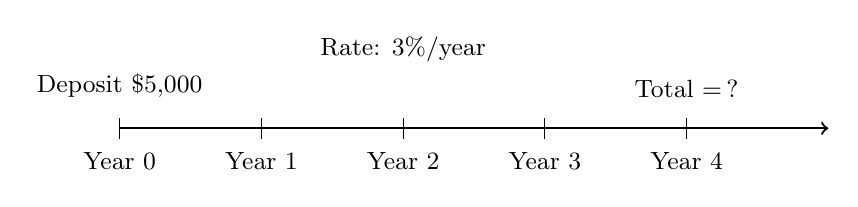
\begin{tikzpicture}[scale=0.9]
  \draw[thick,->] (0,0) -- (10,0);
  \foreach \x/\lab in {0/Year 0, 2/Year 1, 4/Year 2, 6/Year 3, 8/Year 4} {
    \draw (\x,-0.15) -- (\x,0.15);
    \node[below,font=\small] at (\x,-0.2) {\lab};
  }
  \node[above,font=\small] at (0,0.3) {Deposit $\$5{,}000$};
  \node[above,font=\small] at (4,0.8) {Rate: $3\%$/year};
  \node[above,font=\small] at (8,0.3) {Total $= \,?$};
\end{tikzpicture}
\end{center}
\end{questionText}
\correctAnswer{$\$5{,}600$}
\explanation{$I = 5{,}000 \times 0.03 \times 4 = \$600$. Total: $5{,}000 + 600 = \$5{,}600$.}
\end{practiceQuestion}

\begin{practiceQuestion}{m-2-6-q26}{gsa}
\begin{questionText}
The table compares a savings account and a loan. How much net interest does the person earn (interest earned minus interest paid)?

\begin{center}
\begin{tabular}{|l|c|c|c|}
\hline
 & \textbf{Amount} & \textbf{Rate} & \textbf{Time} \\
\hline
Savings & $\$3{,}000$ & $4\%$ & $2$ years \\
\hline
Loan & $\$1{,}000$ & $6\%$ & $2$ years \\
\hline
\end{tabular}
\end{center}
\end{questionText}
\correctAnswer{$\$120$}
\explanation{Savings interest: $3{,}000 \times 0.04 \times 2 = \$240$. Loan interest: $1{,}000 \times 0.06 \times 2 = \$120$. Net: $240 - 120 = \$120$.}
\end{practiceQuestion}

\begin{practiceQuestion}{m-2-6-q27}{gsa}
\begin{questionText}
The bar graph shows the interest earned per year on a $\$6{,}000$ deposit. Each year earns the same interest. How many years does it take to earn $\$900$ total?

\begin{center}
\begin{tikzpicture}[scale=0.55]
  \draw[thick,->] (0,0) -- (0,4.5) node[above]{\small Interest (\$)};
  \draw[thick,->] (0,0) -- (5,0);
  \fill[funBlue!60] (1,0) rectangle (2.5,3);
  \node[below,font=\small] at (1.75,0) {Year 1};
  \node[above,font=\small] at (1.75,3) {$\$150$};
  \foreach \y/\lab in {1/50,2/100,3/150,4/200} {
    \draw (-0.1,\y) -- (0.1,\y) node[left,font=\small,xshift=-2pt] {\lab};
  }
  \node[font=\small] at (3.5,2) {Same each year};
\end{tikzpicture}
\end{center}
\end{questionText}
\correctAnswer{$6$ years}
\explanation{Each year: $\$150$. To reach $\$900$: $900 \div 150 = 6$ years.}
\end{practiceQuestion}
